\documentclass{standalone}
\usepackage{tikz}
\usetikzlibrary{patterns, positioning}
\usepackage[sfdefault]{ClearSans} %% option 'sfdefault' activates Clear Sans as the default text font
\usepackage[T1]{fontenc}

\begin{document}
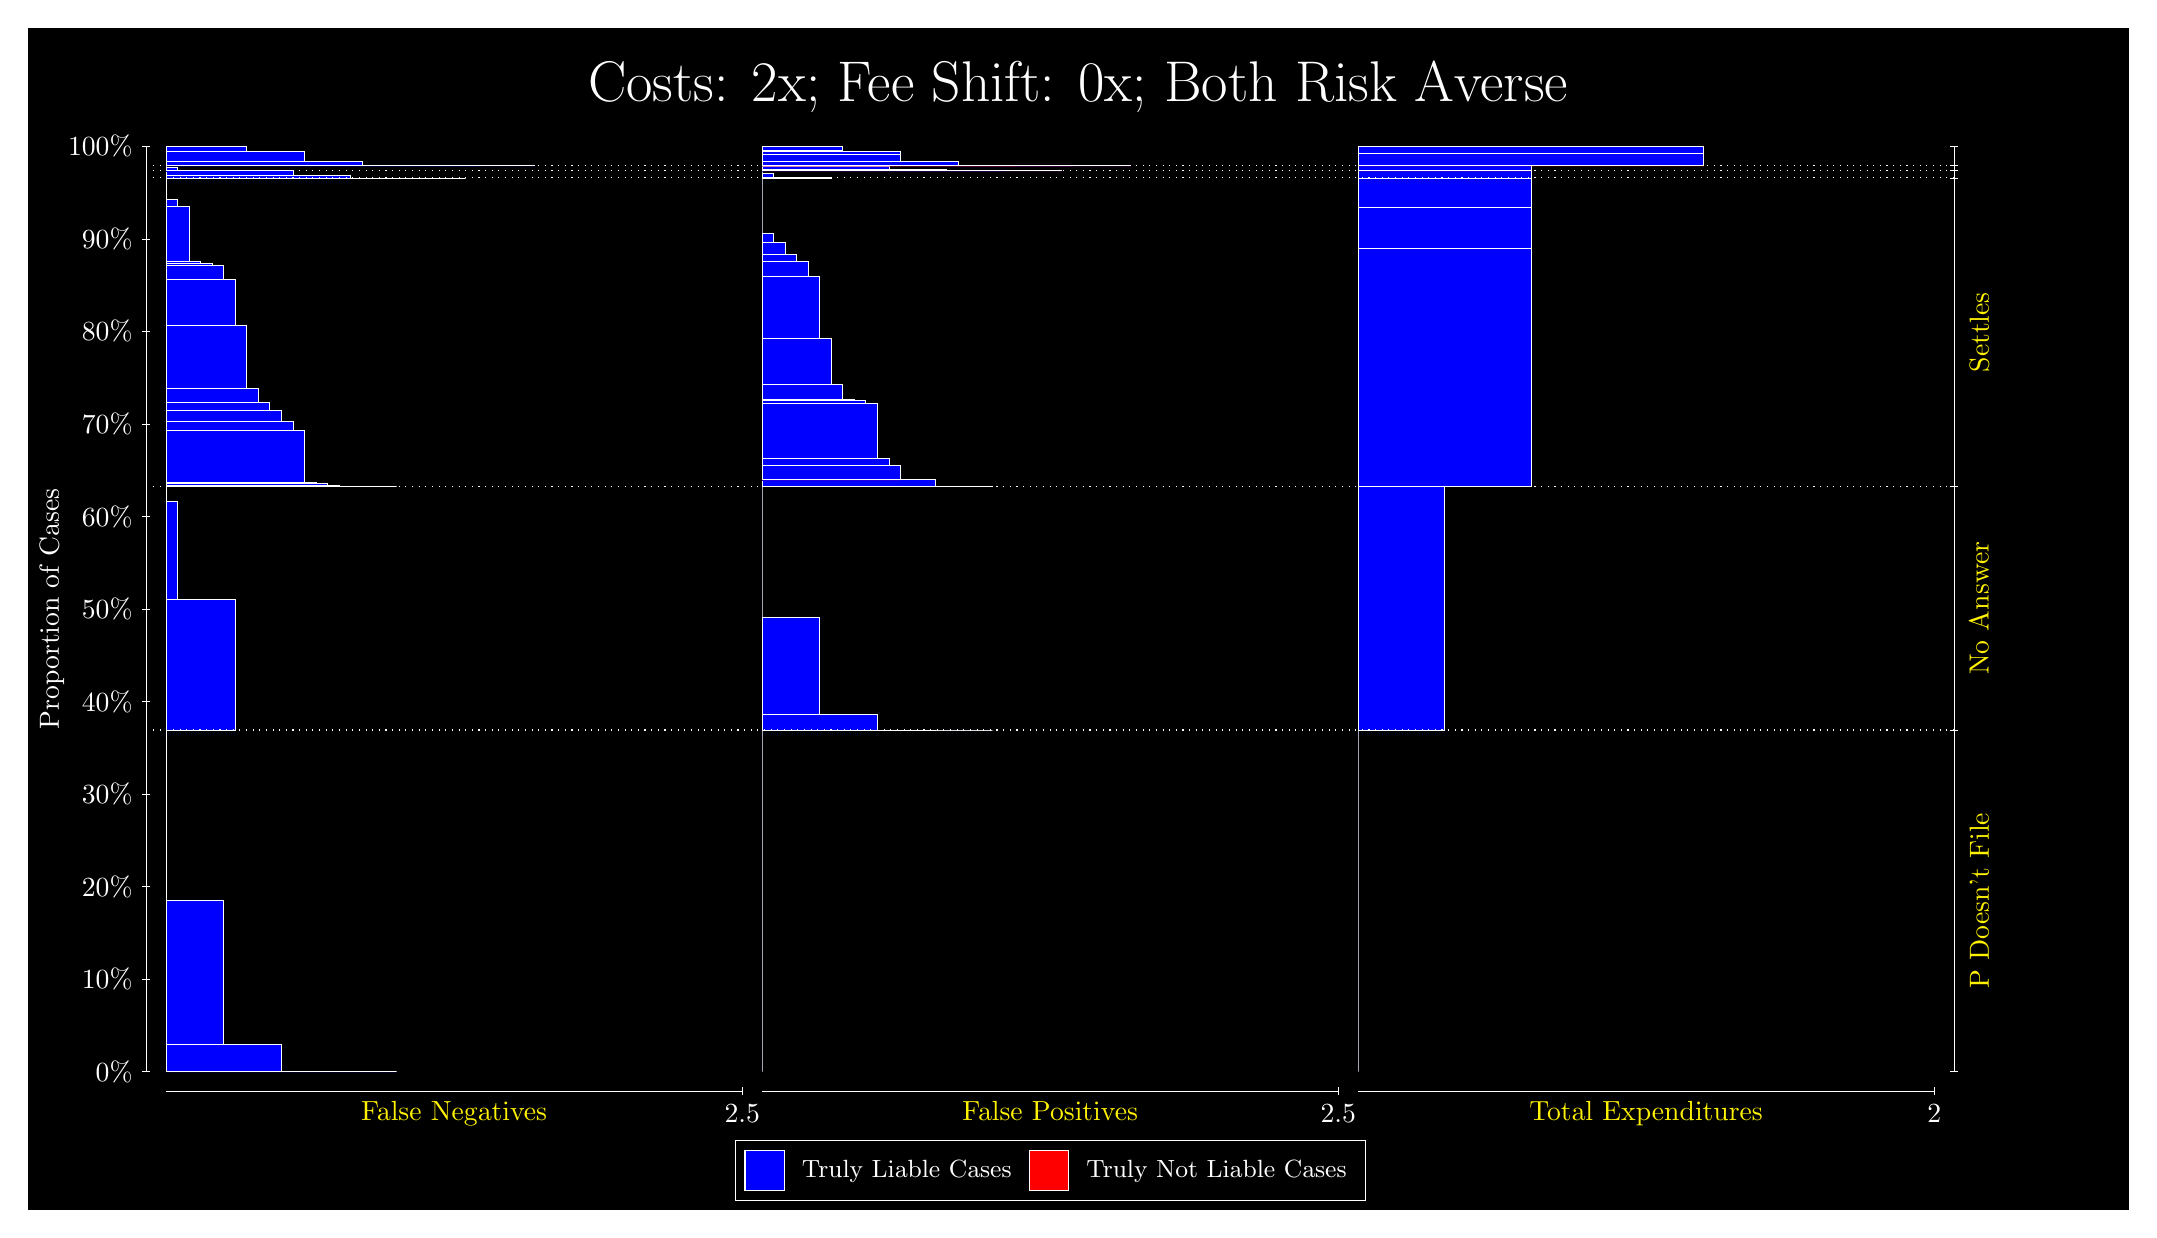
\begin{tikzpicture}
\draw[fill=black] (0,0) rectangle (26.667,15);
\draw[text=white] (0,13.5) rectangle (26.667,15) node[midway] {\huge Costs: 2x; Fee Shift: 0x; Both Risk Averse};
\draw[white, very thin] (1.5,1.75) -- (1.5,13.5);
\node[rotate=90, text=white, anchor=center] at (0.3, 7.625) {Proportion of Cases};
\draw[white, very thin] (1.45,1.75) -- (1.55,1.75);
\node[text=white, anchor=east] at (1.45, 1.75) {0\%};
\draw[white, very thin] (1.45,2.925) -- (1.55,2.925);
\node[text=white, anchor=east] at (1.45, 2.925) {10\%};
\draw[white, very thin] (1.45,4.1) -- (1.55,4.1);
\node[text=white, anchor=east] at (1.45, 4.1) {20\%};
\draw[white, very thin] (1.45,5.275) -- (1.55,5.275);
\node[text=white, anchor=east] at (1.45, 5.275) {30\%};
\draw[white, very thin] (1.45,6.45) -- (1.55,6.45);
\node[text=white, anchor=east] at (1.45, 6.45) {40\%};
\draw[white, very thin] (1.45,7.625) -- (1.55,7.625);
\node[text=white, anchor=east] at (1.45, 7.625) {50\%};
\draw[white, very thin] (1.45,8.8) -- (1.55,8.8);
\node[text=white, anchor=east] at (1.45, 8.8) {60\%};
\draw[white, very thin] (1.45,9.975) -- (1.55,9.975);
\node[text=white, anchor=east] at (1.45, 9.975) {70\%};
\draw[white, very thin] (1.45,11.15) -- (1.55,11.15);
\node[text=white, anchor=east] at (1.45, 11.15) {80\%};
\draw[white, very thin] (1.45,12.325) -- (1.55,12.325);
\node[text=white, anchor=east] at (1.45, 12.325) {90\%};
\draw[white, very thin] (1.45,13.5) -- (1.55,13.5);
\node[text=white, anchor=east] at (1.45, 13.5) {100\%};

\draw[white, very thin] (24.457,1.75) -- (24.457,13.5);
\draw[white, very thin] (24.407,1.75) -- (24.507,1.75);
\node[anchor=west] at (24.407, 1.75) {};
\draw[white, very thin] (24.407,6.0875) -- (24.507,6.0875);
\node[anchor=west] at (24.407, 6.0875) {};
\draw[white, very thin] (24.407,9.1806) -- (24.507,9.1806);
\node[anchor=west] at (24.407, 9.1806) {};
\draw[white, very thin] (24.407,13.1) -- (24.507,13.1);
\node[anchor=west] at (24.407, 13.1) {};
\draw[white, very thin] (24.407,13.191) -- (24.507,13.191);
\node[anchor=west] at (24.407, 13.191) {};
\draw[white, very thin] (24.407,13.253) -- (24.507,13.253);
\node[anchor=west] at (24.407, 13.253) {};
\draw[white, very thin] (24.407,13.5) -- (24.507,13.5);
\node[anchor=west] at (24.407, 13.5) {};

\draw[white, very thin, fill=blue] (1.75,1.75) rectangle (4.6775,1.75);
\draw[white, very thin, fill=blue] (1.75,1.75) rectangle (3.9457,1.7529);
\draw[white, very thin, fill=blue] (1.75,1.7529) rectangle (3.2138,2.0971);
\draw[white, very thin, fill=blue] (1.75,2.0971) rectangle (2.4819,3.9217);
\draw[white, very thin, fill=red] (1.75,3.9217) rectangle (1.75,3.9217);
\draw[white, very thin, fill=blue] (1.75,3.9217) rectangle (1.75,6.0875);
\draw[white, very thin, fill=blue] (1.75,6.0875) rectangle (2.6283,7.7518);
\draw[white, very thin, fill=blue] (1.75,7.7518) rectangle (1.8964,8.9868);
\draw[white, very thin, fill=red] (1.75,8.9868) rectangle (1.75,8.9868);
\draw[white, very thin, fill=blue] (1.75,8.9868) rectangle (1.75,9.1806);
\draw[white, very thin, fill=blue] (1.75,9.1806) rectangle (4.6775,9.1806);
\draw[white, very thin, fill=blue] (1.75,9.1806) rectangle (4.3848,9.1806);
\draw[white, very thin, fill=blue] (1.75,9.1806) rectangle (4.092,9.1809);
\draw[white, very thin, fill=blue] (1.75,9.1809) rectangle (3.9457,9.1983);
\draw[white, very thin, fill=blue] (1.75,9.1983) rectangle (3.7993,9.2208);
\draw[white, very thin, fill=blue] (1.75,9.2208) rectangle (3.6529,9.2298);
\draw[white, very thin, fill=blue] (1.75,9.2298) rectangle (3.5065,9.8907);
\draw[white, very thin, fill=blue] (1.75,9.8907) rectangle (3.3602,10.003);
\draw[white, very thin, fill=blue] (1.75,10.003) rectangle (3.2138,10.152);
\draw[white, very thin, fill=blue] (1.75,10.152) rectangle (3.0674,10.244);
\draw[white, very thin, fill=blue] (1.75,10.244) rectangle (2.921,10.432);
\draw[white, very thin, fill=blue] (1.75,10.432) rectangle (2.7746,11.222);
\draw[white, very thin, fill=blue] (1.75,11.222) rectangle (2.6283,11.806);
\draw[white, very thin, fill=blue] (1.75,11.806) rectangle (2.4819,11.988);
\draw[white, very thin, fill=blue] (1.75,11.988) rectangle (2.3355,12.011);
\draw[white, very thin, fill=blue] (1.75,12.011) rectangle (2.1891,12.044);
\draw[white, very thin, fill=blue] (1.75,12.044) rectangle (2.0428,12.744);
\draw[white, very thin, fill=blue] (1.75,12.744) rectangle (1.8964,12.831);
\draw[white, very thin, fill=red] (1.75,12.831) rectangle (1.75,12.831);
\draw[white, very thin, fill=blue] (1.75,12.831) rectangle (1.75,13.1);
\draw[white, very thin, fill=blue] (1.75,13.1) rectangle (5.5558,13.1);
\draw[white, very thin, fill=blue] (1.75,13.1) rectangle (4.8239,13.1);
\draw[white, very thin, fill=blue] (1.75,13.1) rectangle (4.092,13.134);
\draw[white, very thin, fill=blue] (1.75,13.134) rectangle (3.3602,13.19);
\draw[white, very thin, fill=blue] (1.75,13.19) rectangle (2.6283,13.191);
\draw[white, very thin, fill=red] (1.75,13.191) rectangle (1.75,13.191);
\draw[white, very thin, fill=blue] (1.75,13.191) rectangle (2.6283,13.192);
\draw[white, very thin, fill=blue] (1.75,13.192) rectangle (1.8964,13.23);
\draw[white, very thin, fill=red] (1.75,13.23) rectangle (1.75,13.23);
\draw[white, very thin, fill=blue] (1.75,13.23) rectangle (1.75,13.253);
\draw[white, very thin, fill=blue] (1.75,13.253) rectangle (6.4341,13.253);
\draw[white, very thin, fill=blue] (1.75,13.253) rectangle (5.7022,13.253);
\draw[white, very thin, fill=blue] (1.75,13.253) rectangle (4.9703,13.257);
\draw[white, very thin, fill=blue] (1.75,13.257) rectangle (4.2384,13.314);
\draw[white, very thin, fill=blue] (1.75,13.314) rectangle (3.5065,13.438);
\draw[white, very thin, fill=blue] (1.75,13.438) rectangle (2.7746,13.496);
\draw[white, very thin, fill=blue] (1.75,13.496) rectangle (2.0428,13.5);
\draw[white, very thin, fill=red] (1.75,13.5) rectangle (1.75,13.5);
\draw[white, very thin, fill=blue] (1.75,13.5) rectangle (1.75,13.5);
\draw[white, very thin, fill=red] (9.3189,1.75) rectangle (9.3189,1.75);
\draw[white, very thin, fill=blue] (9.3189,1.75) rectangle (9.3189,6.0875);
\draw[white, very thin, fill=red] (9.3189,6.0875) rectangle (12.246,6.0875);
\draw[white, very thin, fill=blue] (9.3189,6.0875) rectangle (12.246,6.0875);
\draw[white, very thin, fill=blue] (9.3189,6.0875) rectangle (11.515,6.088);
\draw[white, very thin, fill=blue] (9.3189,6.088) rectangle (10.783,6.2813);
\draw[white, very thin, fill=blue] (9.3189,6.2813) rectangle (10.051,7.5163);
\draw[white, very thin, fill=blue] (9.3189,7.5163) rectangle (9.3189,9.1806);
\draw[white, very thin, fill=red] (9.3189,9.1806) rectangle (12.246,9.1806);
\draw[white, very thin, fill=blue] (9.3189,9.1806) rectangle (12.246,9.1808);
\draw[white, very thin, fill=red] (9.3189,9.1808) rectangle (11.954,9.1808);
\draw[white, very thin, fill=blue] (9.3189,9.1808) rectangle (11.954,9.1808);
\draw[white, very thin, fill=red] (9.3189,9.1808) rectangle (11.661,9.1808);
\draw[white, very thin, fill=blue] (9.3189,9.1808) rectangle (11.661,9.1809);
\draw[white, very thin, fill=blue] (9.3189,9.1809) rectangle (11.515,9.2683);
\draw[white, very thin, fill=red] (9.3189,9.2683) rectangle (11.368,9.2683);
\draw[white, very thin, fill=blue] (9.3189,9.2683) rectangle (11.368,9.2686);
\draw[white, very thin, fill=blue] (9.3189,9.2686) rectangle (11.222,9.2686);
\draw[white, very thin, fill=red] (9.3189,9.2686) rectangle (11.075,9.2686);
\draw[white, very thin, fill=blue] (9.3189,9.2686) rectangle (11.075,9.4492);
\draw[white, very thin, fill=blue] (9.3189,9.4492) rectangle (10.929,9.5362);
\draw[white, very thin, fill=blue] (9.3189,9.5362) rectangle (10.783,10.236);
\draw[white, very thin, fill=blue] (9.3189,10.236) rectangle (10.636,10.269);
\draw[white, very thin, fill=blue] (9.3189,10.269) rectangle (10.49,10.292);
\draw[white, very thin, fill=blue] (9.3189,10.292) rectangle (10.344,10.474);
\draw[white, very thin, fill=blue] (9.3189,10.474) rectangle (10.197,11.058);
\draw[white, very thin, fill=blue] (9.3189,11.058) rectangle (10.051,11.848);
\draw[white, very thin, fill=blue] (9.3189,11.848) rectangle (9.9044,12.036);
\draw[white, very thin, fill=blue] (9.3189,12.036) rectangle (9.758,12.128);
\draw[white, very thin, fill=blue] (9.3189,12.128) rectangle (9.6116,12.277);
\draw[white, very thin, fill=blue] (9.3189,12.277) rectangle (9.4652,12.39);
\draw[white, very thin, fill=blue] (9.3189,12.39) rectangle (9.3189,13.1);
\draw[white, very thin, fill=red] (9.3189,13.1) rectangle (10.197,13.1);
\draw[white, very thin, fill=blue] (9.3189,13.1) rectangle (10.197,13.101);
\draw[white, very thin, fill=blue] (9.3189,13.101) rectangle (9.4652,13.157);
\draw[white, very thin, fill=blue] (9.3189,13.157) rectangle (9.3189,13.191);
\draw[white, very thin, fill=red] (9.3189,13.191) rectangle (13.125,13.191);
\draw[white, very thin, fill=blue] (9.3189,13.191) rectangle (13.125,13.191);
\draw[white, very thin, fill=blue] (9.3189,13.191) rectangle (12.393,13.191);
\draw[white, very thin, fill=blue] (9.3189,13.191) rectangle (11.661,13.214);
\draw[white, very thin, fill=blue] (9.3189,13.214) rectangle (10.929,13.252);
\draw[white, very thin, fill=blue] (9.3189,13.252) rectangle (10.197,13.253);
\draw[white, very thin, fill=red] (9.3189,13.253) rectangle (14.003,13.253);
\draw[white, very thin, fill=blue] (9.3189,13.253) rectangle (14.003,13.253);
\draw[white, very thin, fill=red] (9.3189,13.253) rectangle (13.271,13.253);
\draw[white, very thin, fill=blue] (9.3189,13.253) rectangle (13.271,13.253);
\draw[white, very thin, fill=red] (9.3189,13.253) rectangle (12.539,13.253);
\draw[white, very thin, fill=blue] (9.3189,13.253) rectangle (12.539,13.258);
\draw[white, very thin, fill=blue] (9.3189,13.258) rectangle (11.807,13.314);
\draw[white, very thin, fill=red] (9.3189,13.314) rectangle (11.807,13.314);
\draw[white, very thin, fill=blue] (9.3189,13.314) rectangle (11.807,13.315);
\draw[white, very thin, fill=blue] (9.3189,13.315) rectangle (11.075,13.398);
\draw[white, very thin, fill=red] (9.3189,13.398) rectangle (11.075,13.398);
\draw[white, very thin, fill=blue] (9.3189,13.398) rectangle (11.075,13.439);
\draw[white, very thin, fill=blue] (9.3189,13.439) rectangle (10.344,13.452);
\draw[white, very thin, fill=blue] (9.3189,13.452) rectangle (10.344,13.496);
\draw[white, very thin, fill=blue] (9.3189,13.496) rectangle (9.6116,13.496);
\draw[white, very thin, fill=blue] (9.3189,13.496) rectangle (9.6116,13.5);
\draw[white, very thin, fill=blue] (9.3189,13.5) rectangle (9.3189,13.5);
\draw[white, very thin, fill=red] (16.888,1.75) rectangle (16.888,1.75);
\draw[white, very thin, fill=blue] (16.888,1.75) rectangle (16.888,6.0875);
\draw[white, very thin, fill=red] (16.888,6.0875) rectangle (17.986,6.0875);
\draw[white, very thin, fill=blue] (16.888,6.0875) rectangle (17.986,9.1806);
\draw[white, very thin, fill=red] (16.888,9.1806) rectangle (19.083,9.1806);
\draw[white, very thin, fill=blue] (16.888,9.1806) rectangle (19.083,12.203);
\draw[white, very thin, fill=red] (16.888,12.203) rectangle (19.083,12.203);
\draw[white, very thin, fill=blue] (16.888,12.203) rectangle (19.083,12.732);
\draw[white, very thin, fill=red] (16.888,12.732) rectangle (19.083,12.732);
\draw[white, very thin, fill=blue] (16.888,12.732) rectangle (19.083,13.1);
\draw[white, very thin, fill=red] (16.888,13.1) rectangle (19.083,13.1);
\draw[white, very thin, fill=blue] (16.888,13.1) rectangle (19.083,13.191);
\draw[white, very thin, fill=red] (16.888,13.191) rectangle (19.083,13.191);
\draw[white, very thin, fill=blue] (16.888,13.191) rectangle (19.083,13.253);
\draw[white, very thin, fill=red] (16.888,13.253) rectangle (21.279,13.253);
\draw[white, very thin, fill=blue] (16.888,13.253) rectangle (21.279,13.41);
\draw[white, very thin, fill=red] (16.888,13.41) rectangle (21.279,13.41);
\draw[white, very thin, fill=blue] (16.888,13.41) rectangle (21.279,13.5);
\draw[white, dotted] (1.5,6.0875) -- (24.457,6.0875);
\draw[white, dotted] (1.5,9.1806) -- (24.457,9.1806);
\draw[white, dotted] (1.5,13.1) -- (24.457,13.1);
\draw[white, dotted] (1.5,13.191) -- (24.457,13.191);
\draw[white, dotted] (1.5,13.253) -- (24.457,13.253);
\draw[white, very thin] (1.75,1.5) -- (9.0689,1.5);
\node[text=yellow, anchor=north] at (5.4094, 1.5) {False Negatives};
\draw[white, very thin] (9.0689,1.45) -- (9.0689,1.55);
\node[text=white, anchor=north] at (9.0689, 1.45) {2.5};

\draw[white, very thin] (9.3189,1.5) -- (16.638,1.5);
\node[text=yellow, anchor=north] at (12.978, 1.5) {False Positives};
\draw[white, very thin] (16.638,1.45) -- (16.638,1.55);
\node[text=white, anchor=north] at (16.638, 1.45) {2.5};

\draw[white, very thin] (16.888,1.5) -- (24.207,1.5);
\node[text=yellow, anchor=north] at (20.547, 1.5) {Total Expenditures};
\draw[white, very thin] (24.207,1.45) -- (24.207,1.55);
\node[text=white, anchor=north] at (24.207, 1.45) {2};

\node[text=yellow, centered, rotate=90] at (24.777, 3.9187) {P Doesn't File};
\node[text=yellow, centered, rotate=90] at (24.777, 7.634) {No Answer};
\node[text=yellow, centered, rotate=90] at (24.777, 11.14) {Settles};




\draw (12.978300999999998,1.5) node[draw=none] (baseCoordinate) {};
\begin{scope}[align=center]
        \matrix[scale=0.5, draw=white, below=0.5cm of baseCoordinate, nodes={draw}, column sep=0.1cm]{
            \node[rectangle, draw, minimum width=0.5cm, minimum height=0.5cm, fill=blue] {}; &
            \node[draw=none, font=\small, text=white] (B) {Truly Liable Cases}; &
            \node[rectangle, draw, minimum width=0.5cm, minimum height=0.5cm, fill=red] {}; &
            \node[draw=none, font=\small, text=white] (B) {Truly Not Liable Cases}; \\
            };
\end{scope}

\end{tikzpicture}
\end{document}